\chapter{SONATA/PISHAHANG}
\label{ch:pishahang}

	\section{Configuration requirements}
	\label{sec:Configuration requirements to run Pishahang on a single server or VM}
	\begin{itemize}
		\item Operating System: Ubuntu 16.04 as base image (\hyperlink{name}{http://releases.ubuntu.com/16.04/})
		\item Minimum Requirements: 4GB RAM, 40GB hard disk and a non-root user account
	\end{itemize}
	
	
	\section{OpenStack Installation (Ocata)}
	\label{OpenStack Installation}
	\paragraph{}
	Set up an OpenStack environment using DevStack, which is installed via a configuration file named local.conf. The installation guide can also be found at\\ \hyperlink{name}{https://docs.openstack.org/devstack/latest/} 
	
	\begin{itemize}
		\item Other references 
		\footnote{Refer DevStack heat documentation to enable heat service}
		\footnote{Refer DevStack networking-sfc documentation for service chaining}
	\end{itemize}
	
	\subsection*{Steps of installation:}
	\begin{itemize}
		\item Create a user “stack”
		\begin{lstlisting}
sudo useradd -s /bin/bash -d /opt/stack -m stack
echo "stack ALL=(ALL) NOPASSWD: ALL" | sudo tee /etc/sudoers.d/stack
sudo su - stack
		\end{lstlisting}
		
		\item Clone the devstack repository
		\begin{lstlisting}
git clone https://git.openstack.org/openstack-dev/devstack -b stable/ocata
cd devstack
		\end{lstlisting}
		\newpage
		\item Create and configure the local.conf file\\
		\begin{lstlisting}
[[local|localrc]]
ADMIN\_PASSWORD=password
DATABASE\_PASSWORD=$ADMIN_PASSWORD
RABBIT_PASSWORD=$ADMIN\_PASSWORD
SERVICE\_PASSWORD=$ADMIN_PASSWORD 	
		\end{lstlisting}
		
		
		\item Execute the command
		\begin{lstlisting}
./stack.sh
		\end{lstlisting}
		
		\item After installation check and verify from openstack horizon GUI
		
		Access http://1.2.3.4, replace 1.2.3.4 with the IP address of your host
		Login using user id: admin, password: admin
	\end{itemize}
	
	\section{Pishahang installation}
	\label{sec:Pishahang installation}
	The Below steps of installation are performed from the non-root user account
	
	\begin{itemize}
		\item Installing packages
		\begin{lstlisting}
sudo apt-get install -y software-properties-common
sudo apt-add-repository -y ppa:ansible/ansible
sudo apt-get update
sudo apt-get install -y git ansible
		\end{lstlisting}
		\item Clone repository
		\begin{lstlisting}
git clone https://github.com/CN-UPB/Pishahang.git cd Pishahang/son-install
echo sonata | tee ~/.ssh/.vault_pass
		\end{lstlisting}
		\item Start Installation,
		replace "<your\_ip4\_address>" with the IP address where SONATA should be available.
		\begin{lstlisting}
ansible-playbook utils/deploy/sp.yml -e "target=localhost \ public_ip=<your_ip4_address>" -v 
		\end{lstlisting} 
		\item Verify Installation

Open your browser and navigate to http://public\_ip. Login using the username 
sonata and password 1234. If the installation was successful, you should now see 
the dashboard of the service platform

		\item Installation of son-cli
		The SONATA CLI toolset can also be installed via the Python setup script
		\begin{lstlisting}
git clone https://github.com/sonata-nfv/son-cli.git
cd son-cli
python3 setup.py install
		\end{lstlisting}
		
		\item Test if its working by invoking
		\begin{lstlisting}
son-workspace -h
son-package -h
son-publish -h
son-push -h
son-monitor -h
		\end{lstlisting}
		Reference Link - \hyperlink{name}{https://github.com/sonata-nfv/son-cli\#all-dists-using-setuptools}
	\end{itemize}
	
	
	
	\section{Service Descriptor Packaging and uploading}
	\label{sec:Service Descriptor Packaging and uploading}
	The son-cli is to be installed and son-examples repository to be cloned in the environment.
	\begin{itemize}
		\item Add WIM
		\begin{itemize}
			\item Open your browser and navigate to http://public\_ip
			\item Open the "WIM/VIM Settings" tab
			\begin{figure} [h]
				\centering
				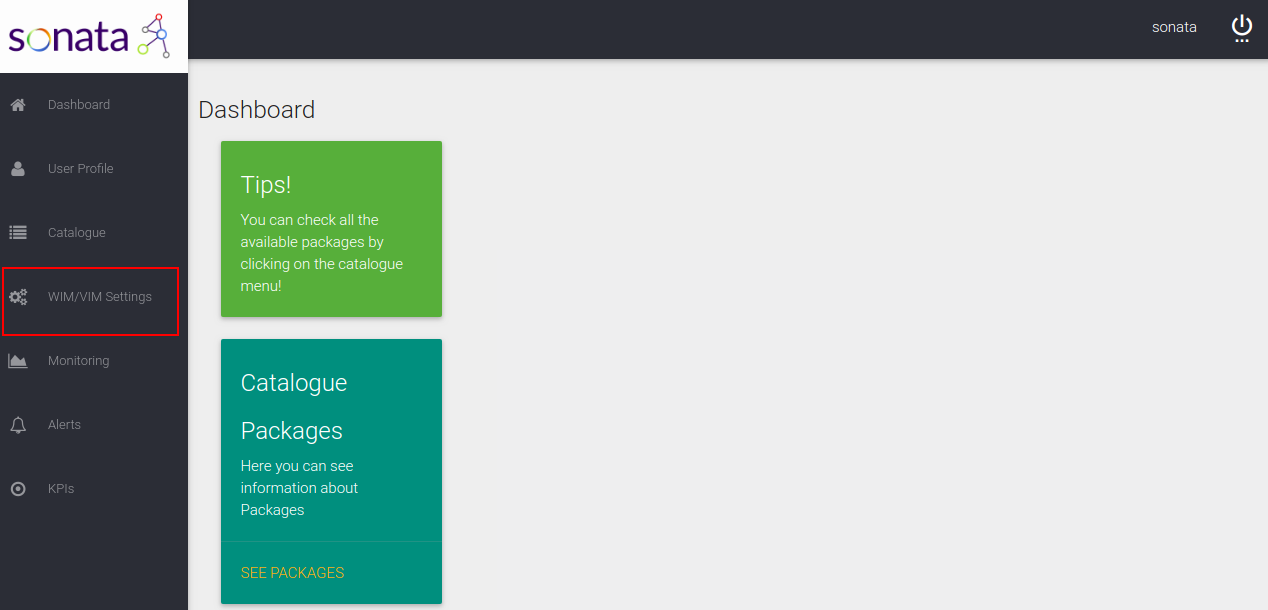
\includegraphics[width=0.7\linewidth]{figures/LinkingStep1}
				\caption{Sonata Dashboard}
				\label{fig:linkingstep1}
			\end{figure}
			
			\item click on add a WIM		
			\item Select "Mock" WIM vendor
			\item Enter any WIM name(e.g. Sonata Test), WIM address(e.g. local host), username(e.g., Sonata) and password(e.g. 1234)
			\item Confirm by clicking "SAVE"
			\begin{figure}[h]
				\centering
				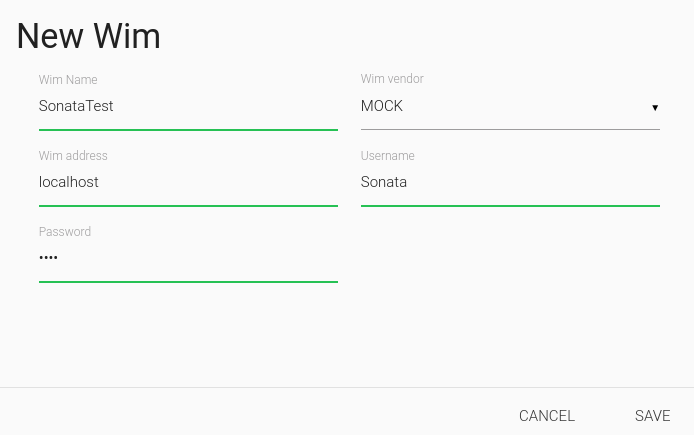
\includegraphics[width=0.7\linewidth]{figures/LinkingStep3}
				\caption{Add WIM}
				\label{fig:linkingstep3}
			\end{figure}
			\newpage
		\end{itemize}
		\item Adding OpenStack VIM
		\begin{itemize}
			\item Click on add a VIM
			\item Enter the VIM name(e.g. DevStack ) , select the WIM just created, enter the country(e.g. germany) and city(Paderborn)
			\item Select ”Heat” VIM vendor
			\begin{figure} [h]
				\centering
				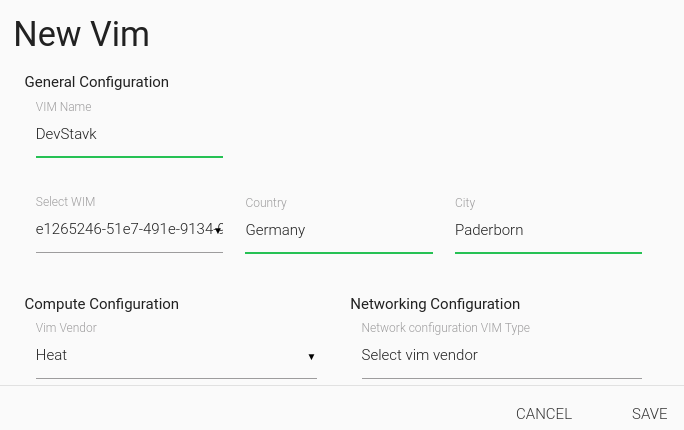
\includegraphics[width=0.7\linewidth]{figures/LinkingStep5}
				\caption{Add VIM}
				\label{fig:linkingstep5}
			\end{figure}
			
			\item Tenant ID: DevStack project id (e.g. sonatademo),Tenant External Netwrok ID: DevStack ID of the public network and Tenant External Router ID: DevStack ID of the router created under sonatademo user i.e. sonata-router as shown below		
			
			\begin{figure}[h]
				\centering
				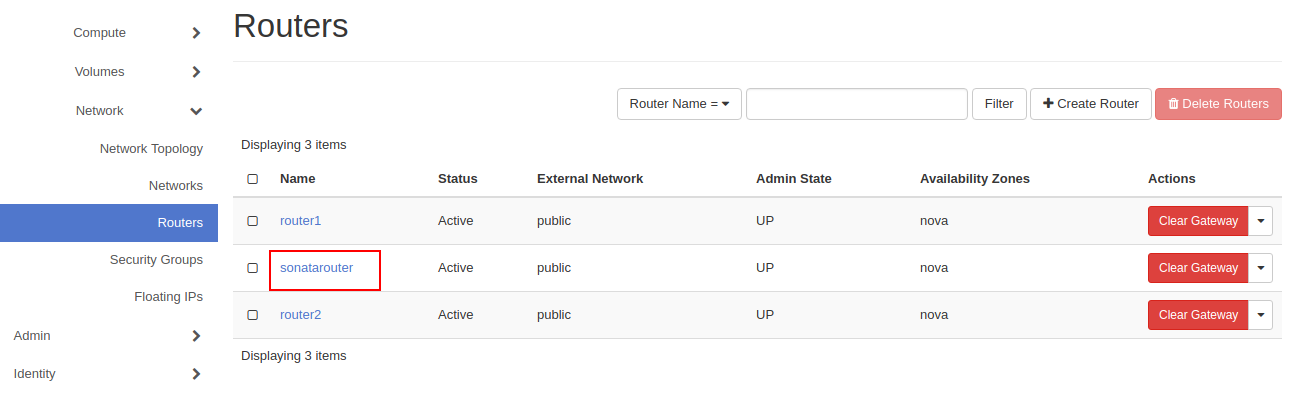
\includegraphics[width=0.8\linewidth]{figures/LinkingStep9}
				\caption{Select Router}
				\label{fig:linkingstep9}
			\end{figure}
			\begin{figure}[h]
				\centering
				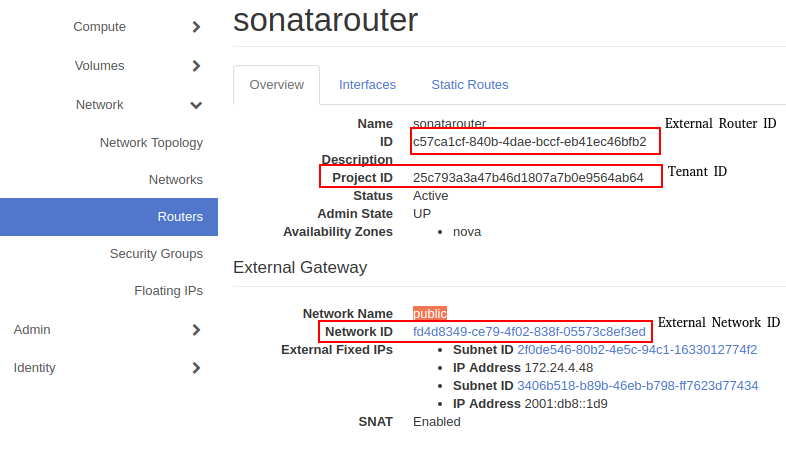
\includegraphics[width=0.9\linewidth]{figures/LinkingStep10}
				\caption{Select IDs}
				\label{fig:linkingstep10}
			\end{figure}
			\newpage
			\item VIM Address: DevStack (131.234.29.34)		
			\item Vim Vendor: “OVS”,Username: sonatademo,Password: password of the user sonatademo (e.g. sonata),Domain: Default
			\item Click on "Save"
			\begin{figure}[h]
				\centering
				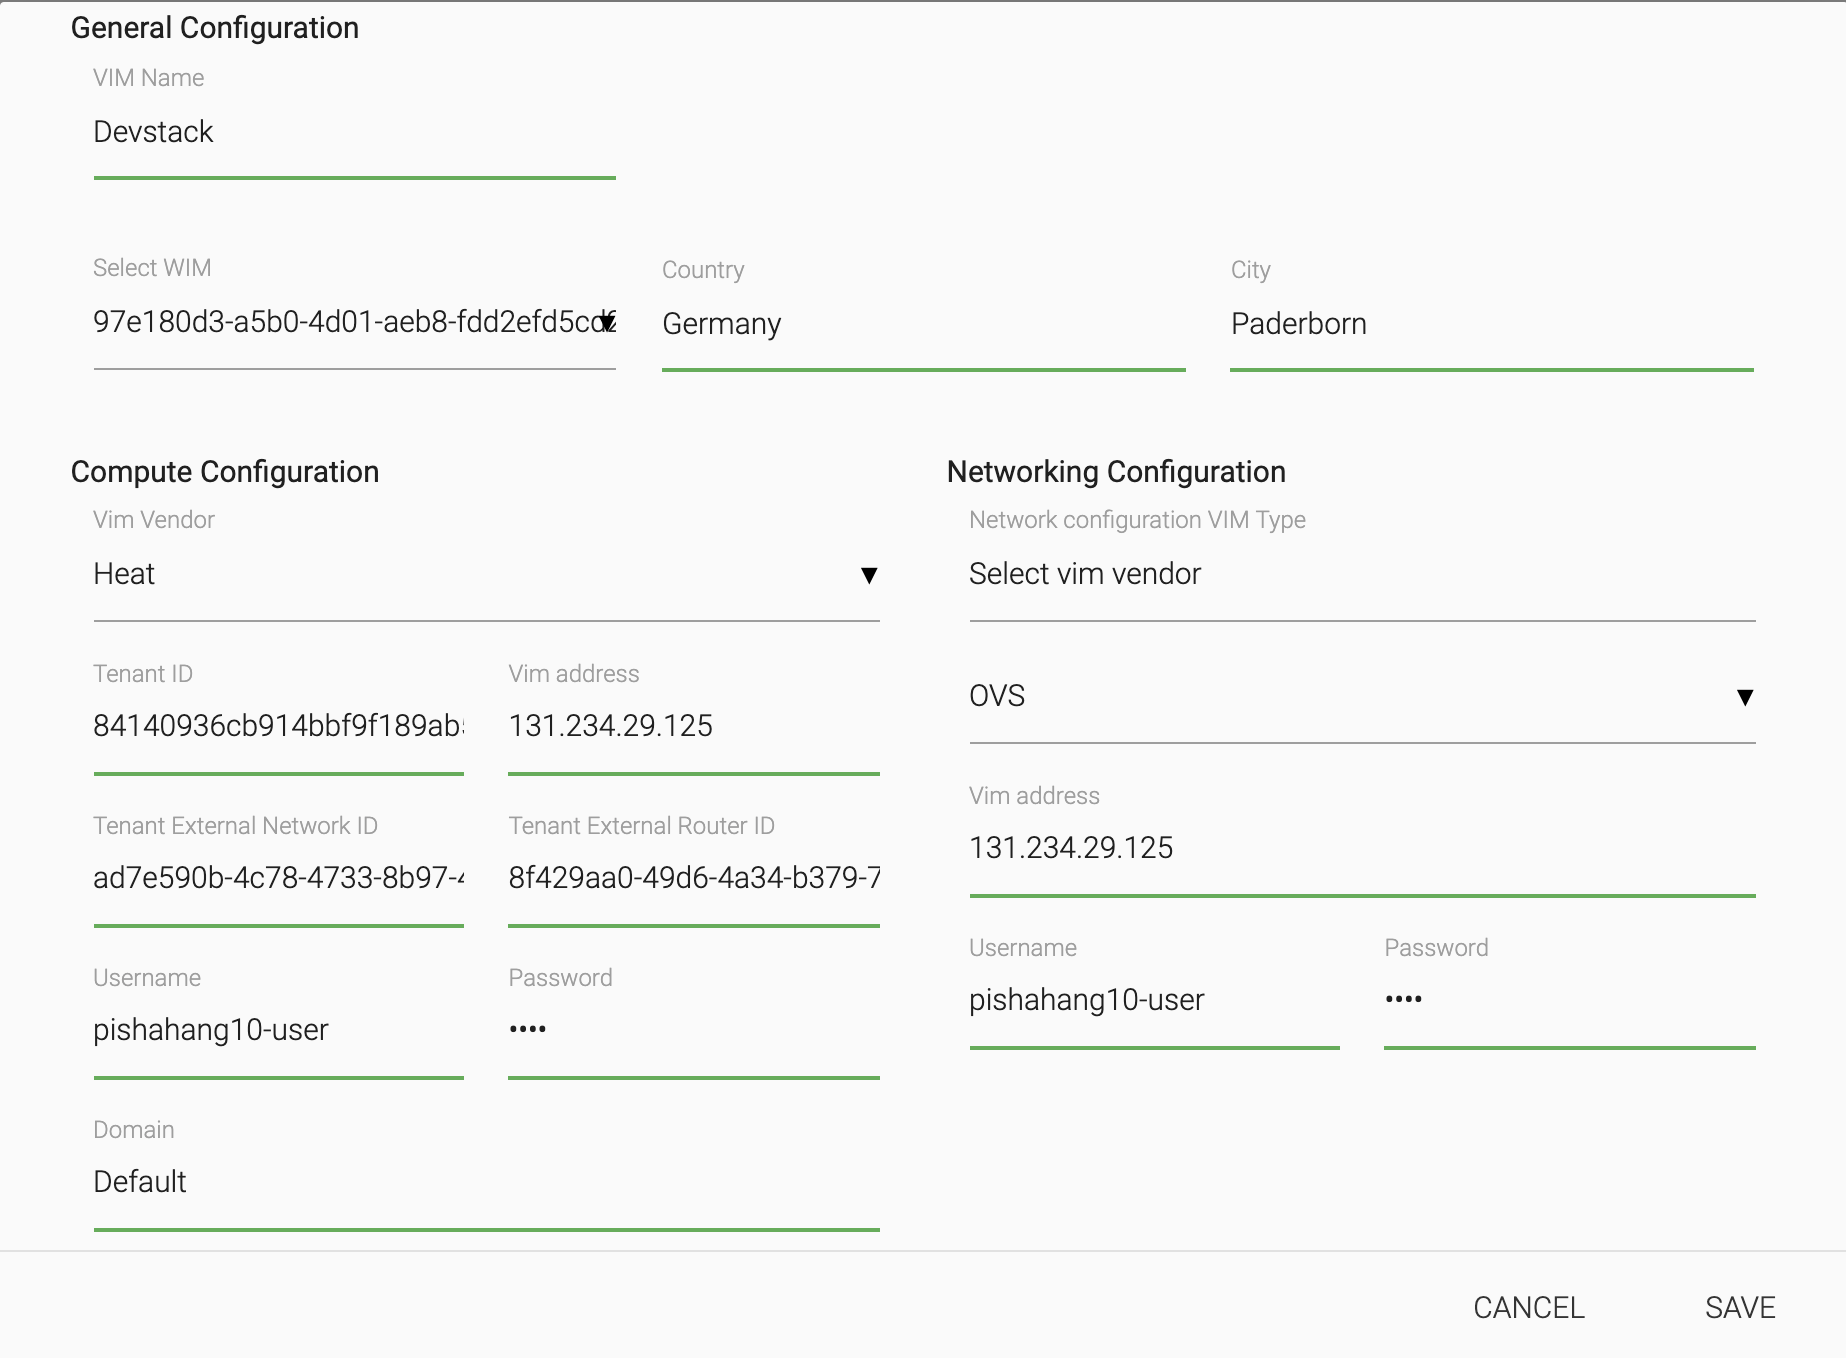
\includegraphics[width=0.7\linewidth]{figures/LinkingStep11}
				\caption{VIM Details}
				\label{fig:linkingstep11}
			\end{figure}
			\newpage	
			\item On-boarding Service Package
			\begin{lstlisting}
git clone  https://github.com/sonata-nfv/son-examples.git
son-workspace --init
son-validate --project  son-examples/service-projects/sonata-demo
son-package --project  son-examples/service-projects/sonata-demo -n \ service_package
son-access config --platform_id ServicePlatform --new --url \ http://131.234.29.102 --default 
son-access auth -u sonata -p 1234
son-access push --upload service_package.son
			\end{lstlisting}
			Reference video - \hyperlink{name}{https://www.youtube.com/watch?v=RsXUIt4rzF0}
		\end{itemize}
		
	\end{itemize}
	
	
	\section{Linking VIM to sonata}
	\label{sec:Linking VIM to sonata}
	Login to the DevStack dashboard: \hyperlink{name}{http://131.234.29.34/dashboard}.There are two users created during installation admin and demo. Password for both users is sonata
	\begin{itemize}
		\item Create New User and Project
		\begin{itemize}
			\item Login as admin user in domain Default and create new user (e.g. sonatademo)
			\item In the menu, go to Identity->User (Create User)
			\item Give the admin role to the new user
			\begin{figure}[h]
				\centering
				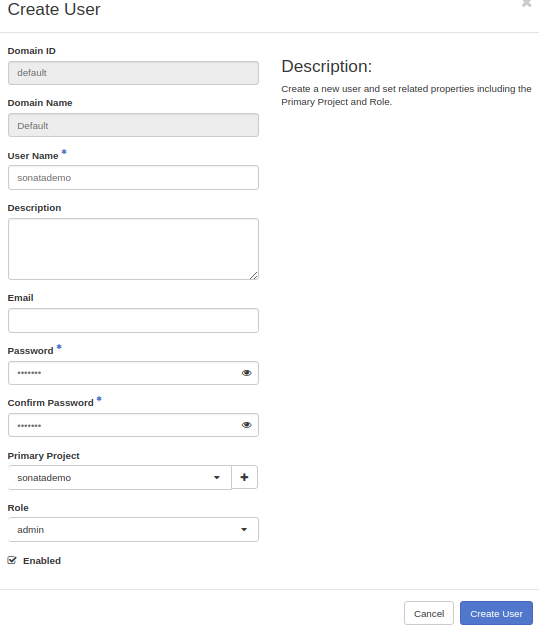
\includegraphics[width=0.7\linewidth]{figures/CreatingUser}
				\caption{Create user}
				\label{fig:creatinguser}
			\end{figure}
			\newpage
		\end{itemize}
		\item Add a new project with the below details
		\begin{itemize}
			\item Project name/tenant name: sonatademo
			\item Allocate maximum number of resources for that project under Quotas tab
			\begin{figure} [h]
				\centering
				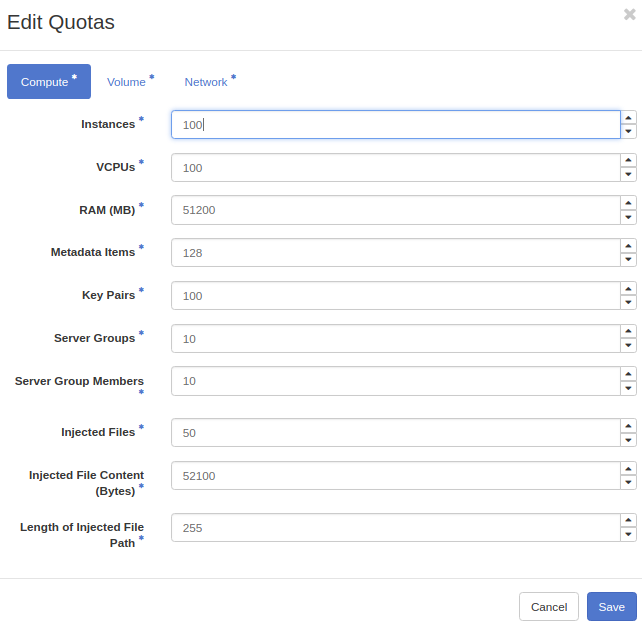
\includegraphics[width=0.7\linewidth]{figures/ProjectQuotas}
				\caption{Edit project quotas}
				\label{fig:projectquotas}
			\end{figure}
			
		\end{itemize}
		\newpage
		\item Create Private Network
		\begin{itemize}
			\item Login as new user(e.g. sonatademo)
			\item Create a network(e.g. sonata-priv) and add the subnet as well (e.g. sonata-priv-sub)
			\item Add the router
			\item Use any private network address, for example 192.168.x.0/24. While creating the router select the External Network as public (Error: Reference source not found). Add the sonata-priv-sub as the interface to the router
			\begin{figure}[h]
				\centering
				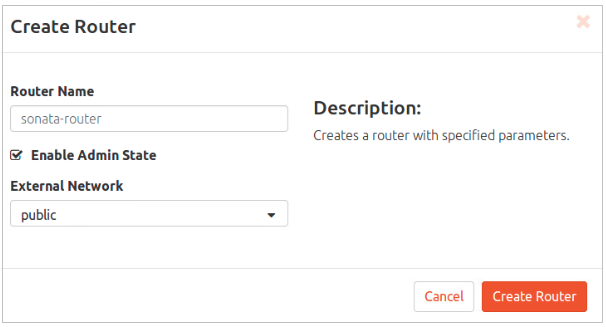
\includegraphics[width=0.7\linewidth]{figures/CreateRouter}
				\caption{Create router}
				\label{fig:createrouter}
			\end{figure}		
		\end{itemize}
	\end{itemize}
	
	\newpage
	
	\section{Onboarding Descriptors}

	NSD can be pushed to the server by using REST API provided by pishahang.
	\begin{itemize}
		\item For CSDs: \hyperlink{name}{http://public\_ip:4002/catalogues/api/v2/csds}
		\item For COSDs: \hyperlink{name}{http://public\_ip:4002/catalogues/api/v2/complex-services}
		\item Dummy NSD that has been uploaded can be seen in the Appendix \ref{ch:Appendix}
	\end{itemize}

	Postman could be used to make the REST calls
	
	1. NSD
	\begin{figure}[H]
		\centering
		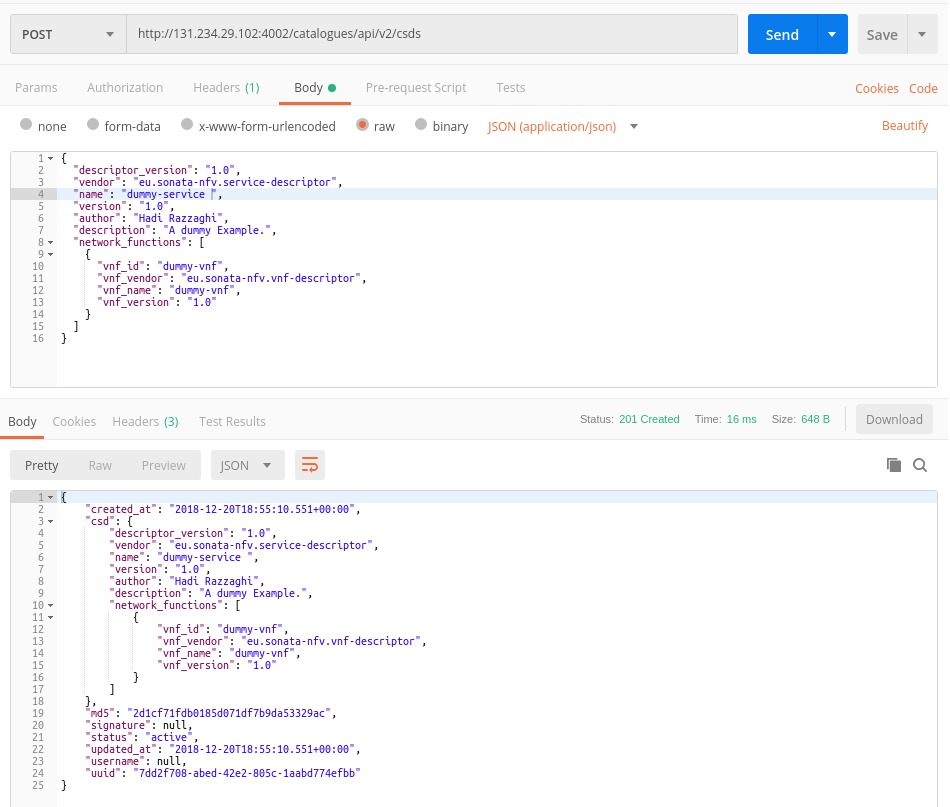
\includegraphics[width=0.7\linewidth]{figures/CSD}
		\caption{REST call for NSD}
		\label{fig:csd}
	\end{figure}
		
	2. VNFD
	
	\begin{figure}[H]
		\centering
		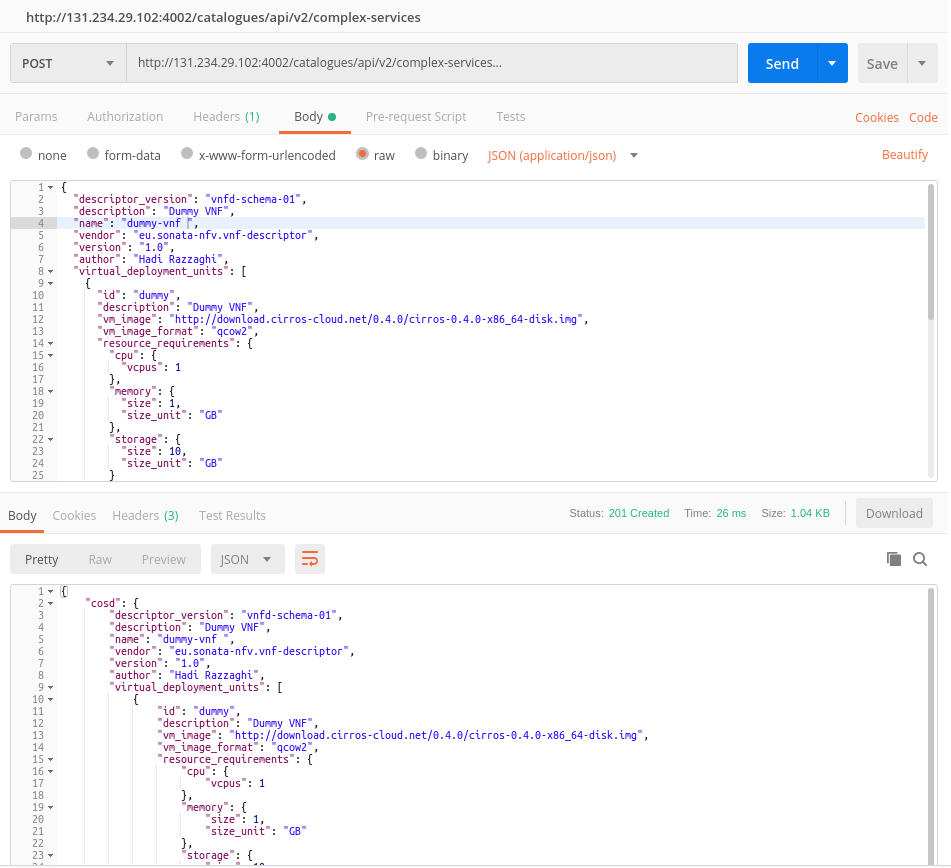
\includegraphics[width=0.7\linewidth]{figures/COSD}
		\caption{REST call for VNFD}
		\label{fig:cosd}
	\end{figure}

	\section{Network Service Instantiation}
	\label{sec:Network Service Instantiation}
	\begin{itemize}
		\item Open your browser and navigate to http://public\_ip:25001
		\item Open the "Available Complex Services" tab
		\item Click the "Instantiate" button of the service you want to deploy
		\item Confirm the instantiate modal (ingress and egress can be empty)
		
	\end{itemize}
	



